% ----------------------------------------
%
% LaTeX Article Template for CUED Reports
% Jon Sowman - 2009
% jon@hexoc.com
% 
% ----------------------------------------
% Set up the document class for an article
\documentclass[11pt]{article}

% Import the required packages for latex
\usepackage{appendix}

% This packages permits using $ \therefore $
\usepackage{amssymb}
\usepackage{graphicx}

% This package allows the use of $ \text{} $
\usepackage{amsmath}
\usepackage{savetrees}

% The document title and author
\title{SB3 - Datalogger\\Cambridge University Engineering Department} 
\author{David Turner \& Jon Sowman}

% Begin the document
\begin{document}
    \maketitle
	
% Insert the abstract for the document here
\begin{abstract}
    A compact, high speed logic analyser is designed with onboard buffering for the simultaneous analysis and logging of up to eight digital channels, one of which may be used as a synchronous clock, for analysis of asynchronous or synchronous transfers. The supporting desktop application is also developed to configure and control the analyser, as well as to retrieve and post-process the recorded data and display it in a convenient format.
\end{abstract}

\section{Hardware Overview}
    A PIC18F4550 microcontroller on a breakout board provides the core of the datalogging hardware, clocked at 48MHz. The USB peripheral external hardware already exists on the board, along with hardware to bring the device out of reset into either the bootloader or user code.

    Additional hardware will be put in place to provide the following functionality:
    \begin{itemize}
    \item Monitor and log up to eight digital channels, optionally synchronised to a clock on one channel
    \item Store up to 1Mbit of data (that is to say, up to 128k samples with up to 8 channels per sample).
    \item Retrieve the samples from memory and transmit them to the desktop computer via USB interface for post processing, analysis and charting.
    \end{itemize}

\subsection{Filtering}
    Frontend antialiasing filters will be put in place to avoid frequency domain aliasing caused by signals at the input above the Nyquist frequency, which will be defined by the sampling frequency of the device. Simple first order low pass RC filters will suffice for this, with a $-3dB$ frequency placed just above the Nyquist frequency.

\subsection{Buffering}
    The data will be captured directly by an SRAM buffer during the logging process, since the PIC does not have enough internal RAM to store a suitable number of samples to satisfy the specification. SRAM, whilst relatively expensive, also demonstrates extremely fast write speeds which is essential to keeping the sampling rate high.

    The hardware of choice is the AS6C1008 1Mbit SRAM IC from Alliance Memory. A 17-bit wide parallel interface is used for byte-addressing, and an 8-bit parallel interface is used for data.

    The address lines will be directly attached to the PIC using the two byte-wide ports PORTB and PORTD, plus one additional line from another port. After the hardware anti-aliasing filters, the eight input channels are connected directly to the SRAM data interface via a 8-way tri-state buffer, controlled by the PIC. This buffer is enabled during the data acquisition phase, and subsequently disabled when the PIC reads back the data from the SRAM.

    Synchronous data capture is possible by the use of the clock input line, which allows one of the input lines to bypass the shift register and be connected directly to the PIC.  The PIC will interrupt on changes of this line and capture data to the SRAM on the appropriate clock edge (set by the user).

\subsection{Data Retrieval}
    Retrieving data from the SRAM is achieved via the use of a parallel-in/serial-out shift register such as the 74HC165 series. The byte-wide parallel input to this device is attached to the data bus, and data is clocked in to the PIC before being packetised and transmitted to the desktop computer via the USB interface.

    A block diagram of the hardware of the data capture system is shown in figure \ref{fig:app}.
    
\subsection{Software Interface}
    The software interface will be constructed using LabWindows and will allow the initiation of datalogging and the viewing of captured data in several formats.  The user can select the asyncronous sample rate or synchronous mode, which channels to capture, and number of samples to capture.  The software will have options to immediately initiate the capture, wait for a trigger byte on the 8 channels, or begin capture on a rising or falling edge of the clock line.  Once the capture is complete and data has been streamed to the PC, it will be available for viewing in both timing diagram and listing formats.  There will be options to display interpret listings in various formats.
    
    \begin{figure}
    \centering
    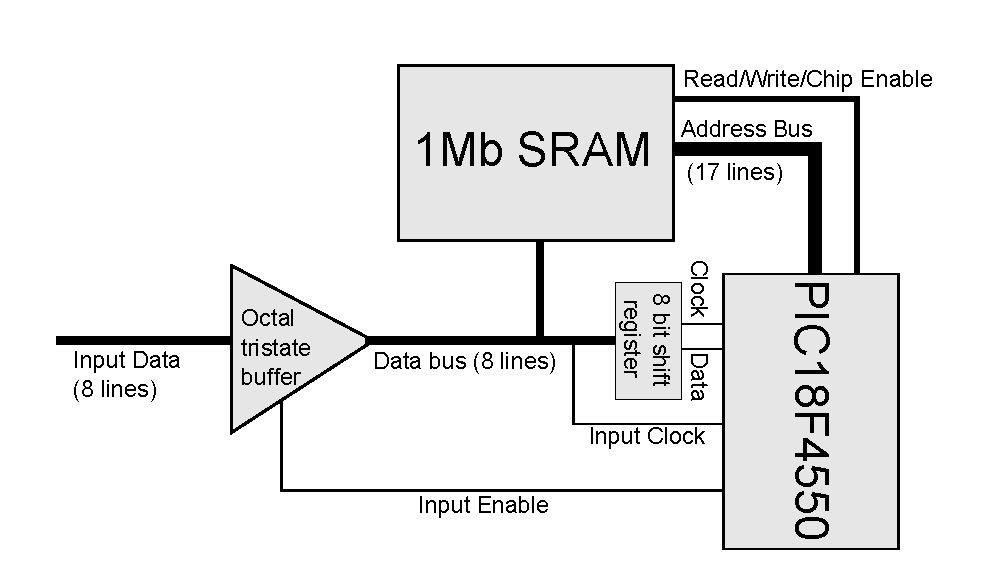
\includegraphics[height=5cm]{block_diagram.pdf}
    \caption{Apparatus setup}
    \label{fig:app}
    \end{figure}
	
% Now print the appendix section
\appendix
\appendixpage
\addappheadtotoc
\section{Appendix 1}
			
\end{document}
